\documentclass[a4paper,11pt,twoside]{article}
\usepackage[utf8x]{inputenc}
\usepackage{geometry}
\usepackage[T1]{fontenc}
\usepackage[english]{babel}
\usepackage{graphicx}
\usepackage{amsmath}
\usepackage{amssymb}
\usepackage{setspace}
\usepackage{fancyhdr}
\usepackage{wrapfig}
\usepackage{subfig}
\usepackage{hyperref}
\usepackage{sidecap}
\usepackage{theorem}
\usepackage{thc}
\usepackage{url}
\usepackage{booktabs}
\usepackage{multirow}
\usepackage{eurosym}
\usepackage{parskip}
\usepackage{indentfirst}
\usepackage{float}
\usepackage[ final ]{pdfpages}
\usepackage[toc,page]{appendix}
\usepackage{mhchem}
\usepackage{breakcites}
\usepackage{titlesec}

\setlength{\parindent}{8mm}
\setlength{\headheight}{15pt}

\geometry{left=2.75 cm,right=2.75 cm, top=3.2 cm, bottom=3.0 cm}
\fancyhf{}
\fancyhead[RO,LE]{\footnotesize{\leftmark}}
\fancyhead[LO,RE]{\thepage}

\pagestyle{fancy}

\renewcommand\maketitle{
\begin{titlepage}

 \begin{center}
 \begin{figure}[htpb]
\rule{1 \textwidth}{1pt}\\
 \smallskip  
 \end{figure}

\vfill

\textbf{ \begin{huge}
Teeth segmentation
\end{huge}}

\vspace{0.4cm}

\begin{Large}
 \textit{Computer vision}
\end{Large}

\vspace{1cm}


\begin{tabular}{ccc}
\LARGE{Rafael Mestre Castillo} \vspace{0.15cm}\\
\large{\textit{Erasmus Mundus Master in Nanoscience and Nanotechnology}}\vspace{0.15cm}\\
\large{KU Leuven}
\end{tabular}
\vspace{1cm}



  


\includegraphics[width=0.33\textwidth]{KULeuven.png}\\
\vspace{0.9cm}
\Large{16th of July, 2015}

\end{center}

\vspace{0.4cm}




\vfill


  \begin{center}
 \rule{1 \textwidth}{1pt}\\
 \end{center}



\end{titlepage}}

\begin{document}




 \maketitle
\tableofcontents
\pagenumbering{gobble}
\newpage
\setcounter{page}{1}
\raggedbottom
\pagenumbering{arabic}


\section{Introduction}\label{Introduction}

Dental radiographs are regarded as one of the best tools for postmortem identification of humans \cite{zhou} \cite{jain}. Teeth can withstand many tragic events and do not suffer from deterioration, as  body tissues do. Furthermore, they present unique features across individuals that can be used for identification purposes. In forensic dentistry, a postmortem dental record is compared to an antemortem dental record. Traditionally, this was done by forensic experts in a manual fashion and that is why an automated method is highly desired. In fact, in 1997, the American Federal Bureau of Investigation (FBI) created a Dental Task Force (DTF) to promote the establishment of an Automated Dental Identification System (ADIS) \cite{shah}. In this context, ADIS is expected to provide automated search and feature matching of teeth in dental X-ray images. Teeth segmentation is a crucial step in this process, but it is a very difficult task due to shape and intensity variations in radiographs \cite{sherif}. The unique features (presence/absence of teeth, crown, pathologies, dental restorations) need to be correctly identified and segmented in order to achieve a good number of matches and a positive identification. An automatic procedure should be able to compare postmortem records with antemortem records and determine the dental radiographs that present the closest matches. Then, if the algorithm cannot achieve a fully reliable identification, a manual system (human-driven) could perform the last steps of the process by correctly identifying the closest match from the small selection of the automated system. A tremendous reduction of the time required for dental identification in forensic dentistry will be achieved, even with a semi-automated model. 

In this report an automated model for segmentation of the upper and lower incisors from a dental radiograph is presented. The aim of this project is to find a fast, reliable and simple method that can segment each one of the 8 incisors keeping its features (position, morphology). However, this method is optimized for standard, regular teeth. Since many jaws present different pathologies, absence of teeth or dental restorations, the method cannot be expected to yield satisfactory results in every case.

For this purpose, 30 different images of dental radiographs were used. For the first 14 images, which during the whole project were solely used as training samples, 40 landmarks per incisor were selected. The rest of the images were used to test the algorithm finding proper segmentations of the teeth. Even though all of the jaws were properly centered in the radiographs, this might not always be the case. In section \textsection\ref{global}, a method for globally localizing the position of the jaw in a radiograph is presented. Section \textsection\ref{centralTeeth} introduces a fast algorithm for the segmentation of the central teeth (incisors) of the person's jaw and section \textsection\ref{ASM} deals with an Active Shape Model (ASM) approach used for the individual segmentation of the 8 teeth. Finally, in section \textsection\ref{discussion} a discussion and evaluation of the method is carried out and section \textsection\ref{conclusions} reports the conclusions and hints at the possible improvements and future work.




\section{Global localization}\label{global}

Radiographs can be local, when the medical specialist is aiming at one specific location of the person's body, or global, when a more general image of several areas are needed. We cannot assure that all of the radiographs that are provided for a teeth segmentation procedure will be localized in exactly the same spot, and therefore it is necessary a technique for recognizing and centering the jaw of a person in different kinds of radiographs. For that purpose, a program based on image recognition techniques was developed in order to localize and crop the jaw in a dental radiograph. Since this is only the initial step, the following approach was taken in order to keep it as simple as possible.

\begin{itemize}
\item A positive database for jaw images and a negative database for non-jaw images were created. The positive database consisted of 14 pictures of jaws taken from the first 14 out of the 30 provided radiographs. The negative database was formed out of 64 pictures of non-jaw elements, such as blurry sections of the radiograph or lateral parts of the jaw. A rescaling of the images to a size of 210x100 was performed.
\item For both the positive and negative pictures, a principal component analysis (PCA) was carried out. For the positive database, a total of 8 components were kept -- for the negative one, the number was 14, in order to prevent false positives.
\item The radiographs used for testing of the program were also resized to a lateral width of 300 pixels and a height that respected the aspect ratio.
\item A window of the same size of the database images, 210x100, was constructed and used in a sliding window search in order to recognize the position of the jaw. In each step, the window image was projected and reconstructed from the multidimensional space spanned by the positive and negative images.
\item A very simple classifier was constructed. The Euclidean norms of the reconstructed images with respect to the original image were taken. The image was considered to be jaw or non-jaw, depending on the norm with the smaller value.
\item Finally, all the detections were clustered in one single window and the resulting image was cropped and saved.
\end{itemize}

As it was mentioned, this approach has the advantages of being very simple, and not very time-consuming. One of the reasons of it is the rescaling of both the database and target images. It was proven that, since the features of a jaw are quite distinctive, using images of smaller size still produced satisfactory results -- the consequent loss of information was not that large. The cropped positive pictures did not need to be of the same size to be used thanks to this rescaling, but a similar aspect ratio for all of them was required. 

The step size of the sliding window was chosen to be 8 pixels. Other values were also tested, such as 3, 5, 10 and 15 pixels. It could be seen that smaller pixel size than 8 did not provide much better results. Larger steps also segmented the jaw properly, but the centering of the image was not that accurate in those cases. For that reason, a step of 8 pixels was used. 

Multiple recognition was unavoidable, specially with small step sizes. For that purpose, different approaches were used in order to cluster the detections into one single point, trying to minimize the complexity, and therefore the time spent in the process. The simplest one consisted in taking the median of all of the detections as an average. The mean was not used since it is very sensitive to extreme values, and the median would solve the problem of  wrong and isolated detections in the edges of the image. Another approach was clustering the edge of the found rectangles by looking at the closest points around them. If the next detection was at distance smaller than a specified value, both of the rectangles were clustered together in the middle point between them. The pair-wise comparison would go on until every point was compared. Naturally, this approach was highly dependent on the starting point, developing different results. After applying this method, multi-detections could still remain that would need to be addressed by taking the mean or the median. Finally, in order to find a more accurate method, a further approach was implemented, based on the affinity propagation clustering algorithm. The advantage of this algorithm resides in the fact that it does not require the number of clusters in advance, but they were provided after it was implemented. However, this method tends to give a large number of clusters and taking the median of the output was compulsory. Since none of the applied approaches gave significantly more accurate products than simply taking the median of all the multi-detections, this one was finally implemented, obtaining satisfactory results. Figure \ref{jawDetections} shows an example of final detections with the different clustering methods.

\begin{figure}
\centering
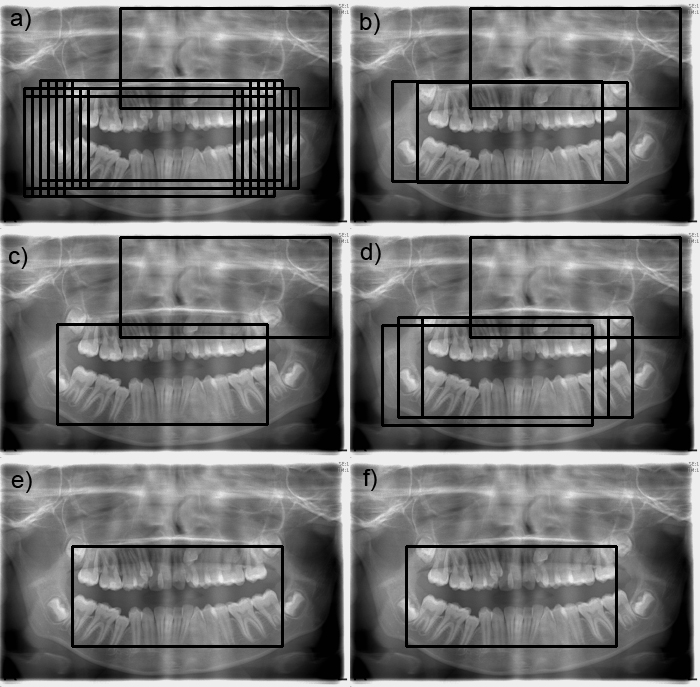
\includegraphics[width=0.75\columnwidth]{jawDetections.jpg}
\caption{Jaw detections for the test image number 22. This was the only image with a different size than the rest. The non-centered position of the jaw points out the necessity of using an image recognition technique. a) Multiple recognitions after the sliding window. Notice the false positive. b) Clustering of the windows by pair-wise comparison, starting from the closest window to the origin and c) starting from the furthest one. This method does not remove an isolated false positive. d) Cluster centers found with the affinity propagation clustering and e) the result after taking the median of the clusters' positions. f) Final detection taking the median of the positions of the windows in a). This method was eventually used due to its simplicity and good results.}
\label{jawDetections}
\end{figure}

This global detection algorithm could be easily improved by adding pyramid representation. This technique allows the application of object detection at different sizes, since the input image might be not properly scaled with respect to the positive database. This can be easily implemented by sub-sampling the input image at different scales and performing the object recognition with a sliding window. Multiple detections will be found at particular scales and a clustering algorithm can be carried out afterwards. In this case, pyramid search was not used simply because it was not necessary at all. The 30 provided images had approximately the same width and height and the size of the window could be chosen by hand. In fact, in this particular case, global detection was not actually necessary, since most of the images were already properly localized and the jaws were situated exactly at the center. Only sample 22, displayed in Figure \ref{jawDetections}, had a different size than the rest, and just using the center of the image to crop would have not been very useful here. Therefore, it is very important to understand that in many occasions this could be the case, and it is crucial for the following steps to have localized jaws of approximately the same size. This method has proven to yield satisfactory results taking into account its simplicity and speed.



\section{Central teeth segmentation}\label{centralTeeth}

Active shape models usually need a good starting point in order to converge to the actual shape that they want to represent. For that reason, we could think of taking the center of the image, or a point nearby, as the starting position for our active shape model. However, this would not be an adequate approach, since the global detection of the jaw is never precisely centered at the required position. Furthermore, some radiographs are performed with an open mouth and some others with a closed mouth. The distances between the upper and lower jaw may vary and even the relative position with respect to the exact center, perhaps due to some dislocation of the teeth. It is therefore necessary to find a good segmentation algorithm to separate the upper and lower parts of the mouth and find an optimal starting point for the active shape model. In the first place, the picture needs to be preprocessed in order to obtain a binary image. Not the whole image needs to be preprocessed -- since we can be sure that the point we are looking for is somewhere around the center of the cropped image of the jaw, we can take a squared section right in the center, that contains part of the upper and lower incisors.

\subsection{Preprocessing of the image}

The first usual step in the preprocessing of any radiograph is noise reduction or denoising, in order to remove the noise that is typical from this images. In particular, the non-local means algorithm, implemented by the OpenCV library for Python \cite{openCV}, was used. Local denoising approaches take the mean value of a group of pixels around a target pixel, but the non-local approach takes into account the mean of all the pixels, weighted by the similarity to the target pixel \cite{nonLocalMeans}.

For the task of obtaining a binary image of the central part of the jaw, the approach described by Nomir \textit{et al} \cite{nomir} was used. This approach consists of several steps. First, the edges of the denoised image are detected using Canny edge detection \cite{canny}. Then, morphological dilation is applied to the binary edge with a window of 3x3 pixels and the original picture is masked with new binary edge. Ideally, half of the pixels will belong to teeth areas and the other half to background. After this, iterative thresholding is applied. With this approach, one tries to find an optimized threshold of the image by iteratively calculating the mean gray values of the background and teeth areas, denoted by $\mu_o^k$ and $\mu_B^k$, respectively, where $k$ is the step of the calculation. At each one of the steps of the computation, the mean values and the threshold are calculated as follows:

\begin{gather}
\mu_o^k = \frac{\sum_{(i,j)\in dental} f(i,j)}{\#dental\_pixels},\\
\mu_B^k = \frac{\sum_{(i,j)\in background} f(i,j)}{\#background\_pixels},\\
T_{k+1} = \frac{\mu_B^k + \mu_o^k}{2},
\end{gather}

\noindent
where $f(i,j)$ is the gray scale value of pixel $(i,j)$ and $T_k$ is the calculated threshold at step $k$.

If the threshold does not change after a certain iteration, the process is stopped. The pixels of the original image that are below the threshold values are set to zero, meanwhile the rest are left with the same value. In Figure \ref{adaptive}, it can be seen that the iteratively thresholded image manages to separate the upper and lower jaw in most of the cases but it does not segment the teeth laterally. Figure \ref{thresholding} shows a case in which the thresholding fails and part of the central area is incorrectly taken as teeth. The edge detection worked properly, as can be seen in the same figure, but the original imaged contained a whitened area that had even more intensity than some teeth. In these cases, it is very difficult to separate the jaws by these method, because there is a clear overlap in intensities between the background and teeth interior.

\begin{figure}
\centering
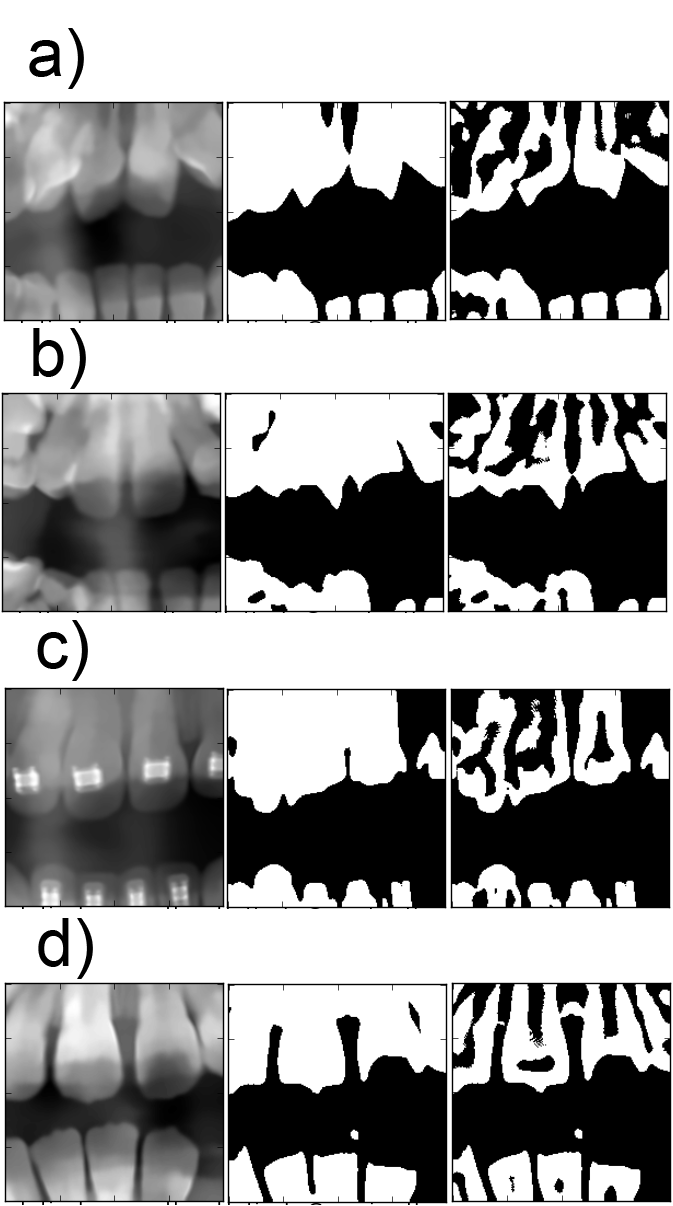
\includegraphics[width=0.65\columnwidth]{adaptive.png}
\caption{a) Test image 19. b) Test image 21. c) Test image 27. d) Test image 28. From left to right: original image after denoising, binary image obtained by iterative thresholding, and binary image obtained after applying adaptive thresholding on the image masked by the iterative thresholding binary picture.}
\label{adaptive}
\end{figure}

\begin{figure}
\centering
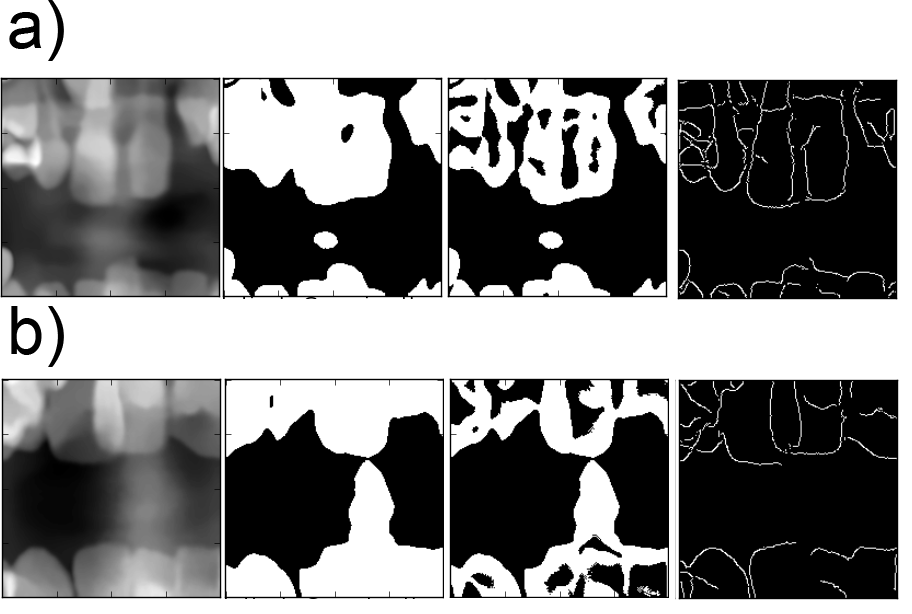
\includegraphics[width=0.65\columnwidth]{thresholding.png}
\caption{a) Test image 16. b) Test image 22. From left to right: original image after denoising, binary image obtained by iterative thresholding, and edges detected by Canny edge detection.}
\label{thresholding}
\end{figure}

As it was mentioned, in many occasions iterative thresholding cannot segment the teeth laterally. To improve the results, adaptive thresholding was performed, as suggested by Nomir \textit{et al} \cite{nomir}. In adaptive thresholding, a window of a certain size is used to calculate the threshold value of the pixels around a certain point. If the value of the central pixel is smaller than this threshold, the pixel is eliminated. A function provided by OpenCV was used and the threshold value was calculated taking the weighted sum of the neighboring values where the weights were given by a Gaussian window. The method was applied on the masked image obtained by the iterative thresholding algorithm. In Figure \ref{adaptive}, it can be seen how this method improves the previous results by laterally segmenting the teeth, although parts of the interior is also taken as background. However, in Figure \ref{thresholding}, we can observe that it does not eliminate the wrong segmentation between the upper and the lower part. 



\subsection{Segmentation of the jaw}\label{centralSegmentation}

Using the binary image of the central part of the image, the upper and lower areas of the jaw were segmented using a simplified model of the one described in \cite{nomir}. In that research, they used a horizontal integral projection defined as

\begin{equation}
H(i)=\sum\limits_{j=1}^n f(i,j),
\end{equation}

\noindent
where $f(i,j)$ is the binary scale value of pixel $(i,j)$ of the $m \times n$ binary image obtained after thresholding. They allowed the image to be rotated over a small angular range in order to account for deviations of the horizontal line.

In this case, we are not that interested in segmenting accurately the upper and lower jaw, but only in finding a that can be called the actual center of the jaw that can be used as a starting point for the active shape model. Furthermore, in all of the samples that were being considered, the separation was sufficiently large to be able to apply this approximation with no problems. Therefore, the horizontal profiles were calculated and only those whose integral projection was below certain value were accepted. Figure \ref{jawSegmentation} shows different cases of jaw segmentation. Obviously, due to the fact that a range of values (not only the minimum of them) were selected, several lines can appear in the image. We can see how sometimes the method works perfectly, but in other occasions it fails to segment the jaw exactly in the middle due to the noise that existed in between and that turned out to be a problem during thresholding. However, in most of the cases this problem was avoided and the segmentation was possible.

\begin{figure}[h]
\centering
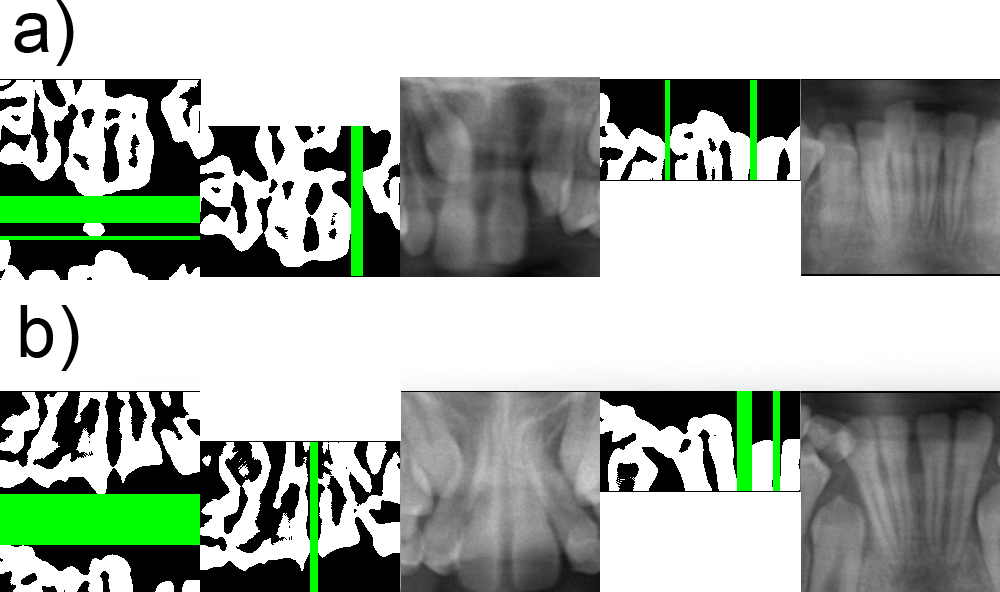
\includegraphics[width=0.95\columnwidth]{jawSegmentation2.png}
\caption{a) Test image 16. b) Test image 21. From left to right: horizontal segmentation of the image obtaiend by adaptive thresholding, vertical separation of the upper incisors, final segmentation of the upper incisors, vertical separation of the lower incisors, and final segmentation of the lower incisors. Notice the difference sizes used in the vertical segmentation of the teeth, in order to avoid tissue regions.}
\label{jawSegmentation}
\end{figure}

Since the separation between upper and lower incisors was sometimes quite large, taking the mean value of the selected horizontal profiles was not  good enough as a starting point. In order to get as close as possible to the upper jaw, the average of the mean value and the value at the higher position was used. For the lower jaw, the average of the mean value and the lower-positioned value was used. With this approach, two problems could be solved. First, segmenting the incisors in a place that was not too far away, due to the large distance between upper and lower parts. Secondly, avoiding a cut across a teeth, since the thresholding algorithm sometimes was not able to recognize the tips of the teeth. 


Lateral separation of the incisors is a much more difficult task, since they are very close together. Adaptive thresholding gets over this difficulty only in certain occasions, but not in all of them. In order to achieve a good location of the center of the incisors, the lower or upper teeth were selected in a small window, taking as a reference point the one obtained by the algorithm just described. Canny edge detection, morphological dilation, iterative thresholding and adaptive thresholding were again performed to obtain a binary image of the corresponding set of teeth. In this occasion, a vertical integral projection was calculated, and the values below a certain threshold were selected. The central position of the incisors was taken as the mean value of all of them which were selected. This approach did not yield good results every time, since the only previous information about the horizontal position of the incisors was an estimated point given by the center of the jaw localized at the beginning.

\section{Active shape model}\label{ASM}

Active shape models are a group of statistical models, developed by Tim Cootes and Chris Taylor \cite{ASM}, in which a model of an object is iteratively deformed to fit a target object in an image. These models make us of a set of training images, from which a point distribution model (PDM) is obtained from a statistical shape analysis of the samples. The shape suggested by the model to best fit the target image is deformed only in ways that are allowed by this PDM. 

For this project,  sets of 40 landmark for each one of the 8 incisors and for each one of the 14 sample images were provided. Before applying the active shape model developed, the landmarks and target image needed to be preprocessed according to the following approach:

\begin{itemize}
\item For one specific tooth (or group of teeth) the whole set of landmarks corresponding to the 14 sample images was loaded into the program. A Procrustes analysis  was performed in order to obtain a PDM of the images. During this process, each set of landmarks is translated to the origin, uniformly scaled, and rotated to a reference angle. 

\item After this, a PCA  was used in order to find the linearly uncorrelated principal components which possess the largest variance of the samples. The number of components were chosen in such a way that they accounted for 99\% of the total variance. 

\item A starting point was provided, depending on the type and total number of teeth to fit. Assuming that the initial point was accurate enough, the original target image was cropped around this point using a window that would contain the teeth of interest.

\item A multi-resolution approach, as suggested by Tim Cootes \cite{ASM2}, was used in order to prevent shapes to converge to a local minimum. Depending on the case, different scaling levels were used. For each scaling level, the target image was denoised and re-sampled to get a coarser structure. A Canny edge detection algorithm with morphological dilation where applied to obtain the edges of the teeth. In this project, level $L=1$ corresponds to the original image, and the images were simply resized as $N_p/L$, where $N_p$ is the total number of pixels in the image.
\end{itemize}

Procrustes analysis also allows the use of mirror images for the shape analysis. In this case, it was chosen not to do so, in order to decrease the computational time. As it will be explained later on, the process was repeated several times for different groups of teeth, and a Procrustes analysis and PCA were necessary for each group. For this project, it was assumed that adding mirror images of the teeth could increase the computational time and the reconstruction capacity of the system would not be extremely improved.

At each one of the scaling levels, the algorithm developed for fitting the shape of the teeth consisted on the following steps:

\begin{enumerate}

\item From the starting point, a mean shape, $\bar{x}$ is situated at a specific position.

\item Using PCA information of the set of landmarks, a reconstruction of the target image is obtained using $\mathbf{x} = \bar{\mathbf{x}} + \mathbf{Pb}$, where $x$ is the reconstructed image, $\mathbf{P}$ are the eigenvectors that contain 99\% of the variance, and $\mathbf{b}$ are the shape parameters.

\item For each landmark of the model shape, an intensity profile of the edge image along its normal direction is calculated. Depending on the scaling level, the length of the profile is calculated to be $L_{profile} = 10 + 16/L$. The pixel with the maximum value in the profile is taken as the next position of the landmark. In the case of several maxima of the same value, the mean position is taken.

\item The displacement vectors of the landmarks are calculated as $d\mathbf{X}_i = \mathbf{L}_i^{(a)} - \mathbf{L}_i^{(b)}$, where $\mathbf{L}_i^{(a)}$ and $\mathbf{L}_i^{(b)}$ are the position of landmark $i$ before and after the calculation of the profile, respectively.

\item The shape parameters adjustments are calculated from the displacement vectors as $d\mathbf{b}=\mathbf{P}^Td\mathbf{X}$.

\item The shape model is reconstructed from this shape parameters, $\mathbf{x} = \bar{\mathbf{x}} + \mathbf{P}d\mathbf{b}$.

\item The newly reconstructed image is rotated, scaled and translated with respect to the form calculated in step 3 (with the landmarks on the maximum edges), so that it minimizes the least squares distances with the method described by Tim Cootes in \cite{ASM}.  

\item Depending on the scaling level, different convergence conditions are used. If convergence is obtained, stop the program or go to the next scaling level, if applicable. If there is no convergence, go to setp 3.

\end{enumerate}

In some cases, the Mahalanobis distance \cite{mahalanobis} is used to find the next position of the landmarks in step 3. This measure of distance calculates the separation between one profile perpendicular to a landmark and a distribution of the same profiles of the 14 training landmarks. The position of the maximum was decided to be used instead due to several reasons. The main reason is the fact that a group of profiles for a certain landmark is not usually found to follow a good distribution. This project aims to find a simple and automated method for teeth segmentation and, as it was mentioned, the preprocessing of the images cannot be individualized in order to find the best parameters for the algorithms. That is why, in some cases, the profiles of a certain landmark across the training samples can be very different. In some cases the edges were not properly found and the profile was 0 in every point. In other cases the noise of the image was wrongly taken as edges and the profile presented random variations. Hence, the profiles of the training landmarks could not be assumed to follow a good distribution, and the approach of taking the maximum value was selected.

This approach, of course, also generates many mistakes. Sometimes, the edge of a contiguous tooth has a greater value than the actual edge of the tooth or there is fuzziness inside or outside that can give a wrong position. This error was intended to be minimized by changing the length of the profile depending on the scaling level. In higher scaling levels (a coarser image), a large number of pixels could make the model scale too much or migrate to the wrong direction, due to the influence of adjacent structures. In the first level of scaling, however, a small number of pixels would not be useful, since the profiles might not contain any information about nearby edges. Therefore, for low levels, the profile length was chosen to be larger, and vice versa for higher levels. Still, these lengths were adapted so that higher scaling levels had a bigger range around the landmarks -- the aim of this multi-resolution approach is the possibility of allowing low resolution cases to scan around a larger amount of pixels so that the shape can migrate to the approximate position of the tooth. That is also why different convergence criteria were used. Since the high scaling level can detect edges around a bigger range, it would be more difficult to find convergence. The criteria were more relaxed for higher levels than for lower levels.

This model was applied several times in order to find a good position for the teeth. This approach turned out to give better results than simply doing it once with the starting point suggested in section \textsection\ref{centralTeeth}. This is due to the feedback that several teeth reconstructions can give to each other based on the fact that their relatives position are quite established. In this project, it was proceeded in the following way:

\begin{enumerate}

\item The four upper incisors were fitted at the same time, using the central point calculated in section \textsection\ref{centralTeeth}. Both Procrustes analysis and PCA were performed for the set of the four teeth kept together in order to find a good approximation of the position of each one of the teeth. Only scaling levels 4 and 3 were used in this case, since we are only interested in a general position.

\item Next, only the two central incisors were fitted, in an attempt to improve the result acquired in the previous step. Therefore, levels 2 and 1 of resolution were used.

\item With the information about the approximated position of the center of each one of the teeth provided by the first two fittings, each one of the four upper incisors were fitted. In order to prevent a great amount of migration from the tooth, only the original image (level 1) was used. 
\end{enumerate}

In these three steps, extensive feedback was employed to improve the position of the teeth. For instance, for the calculation of the position of the second incisor, both the position of the tooth from the fittings in steps 1 and 2 were used. Sometimes one of the two fittings produced a wrong rotation or migration of the landmarks, and taking the mean of both positions helps alleviate this mistake. For the rest of the teeth, feedback from the relative position of all the other teeth is also used. However, it is not always possible to prevent a bad computation of the center in some of the cases. Figure \ref{finalSegmentation} will later show some examples.

For the lower teeth, the same kind of approach is used. This time, both the mean position of the upper teeth and the segmentation realized in section \textsection\ref{centralTeeth} were used to find the best position of the teeth. Next, a fitting of the two central teeth and individual fittings of the rest were performed, using feedback from previous actions. It is important to mention that in many occasions, convergence could not be found quickly. A maximum number of repetitions was set so that the computation time was not too large. Most of the occasions, the shape was found to be stuck in two local nearby positions, going back and forth in every iteration but without changing much the general shape. This is a big drawback of the method, and it is necessary to find a way of eliminating this.

\section{Discussion}\label{discussion}

This algorithm consisted of three main parts: jaw segmentation, central teeth segmentation and active shape model fitting. The recognition and cropping of the jaw was successful in 100\% of the test images. Figure \ref{jaws} show some examples. 

\begin{figure}
\centering
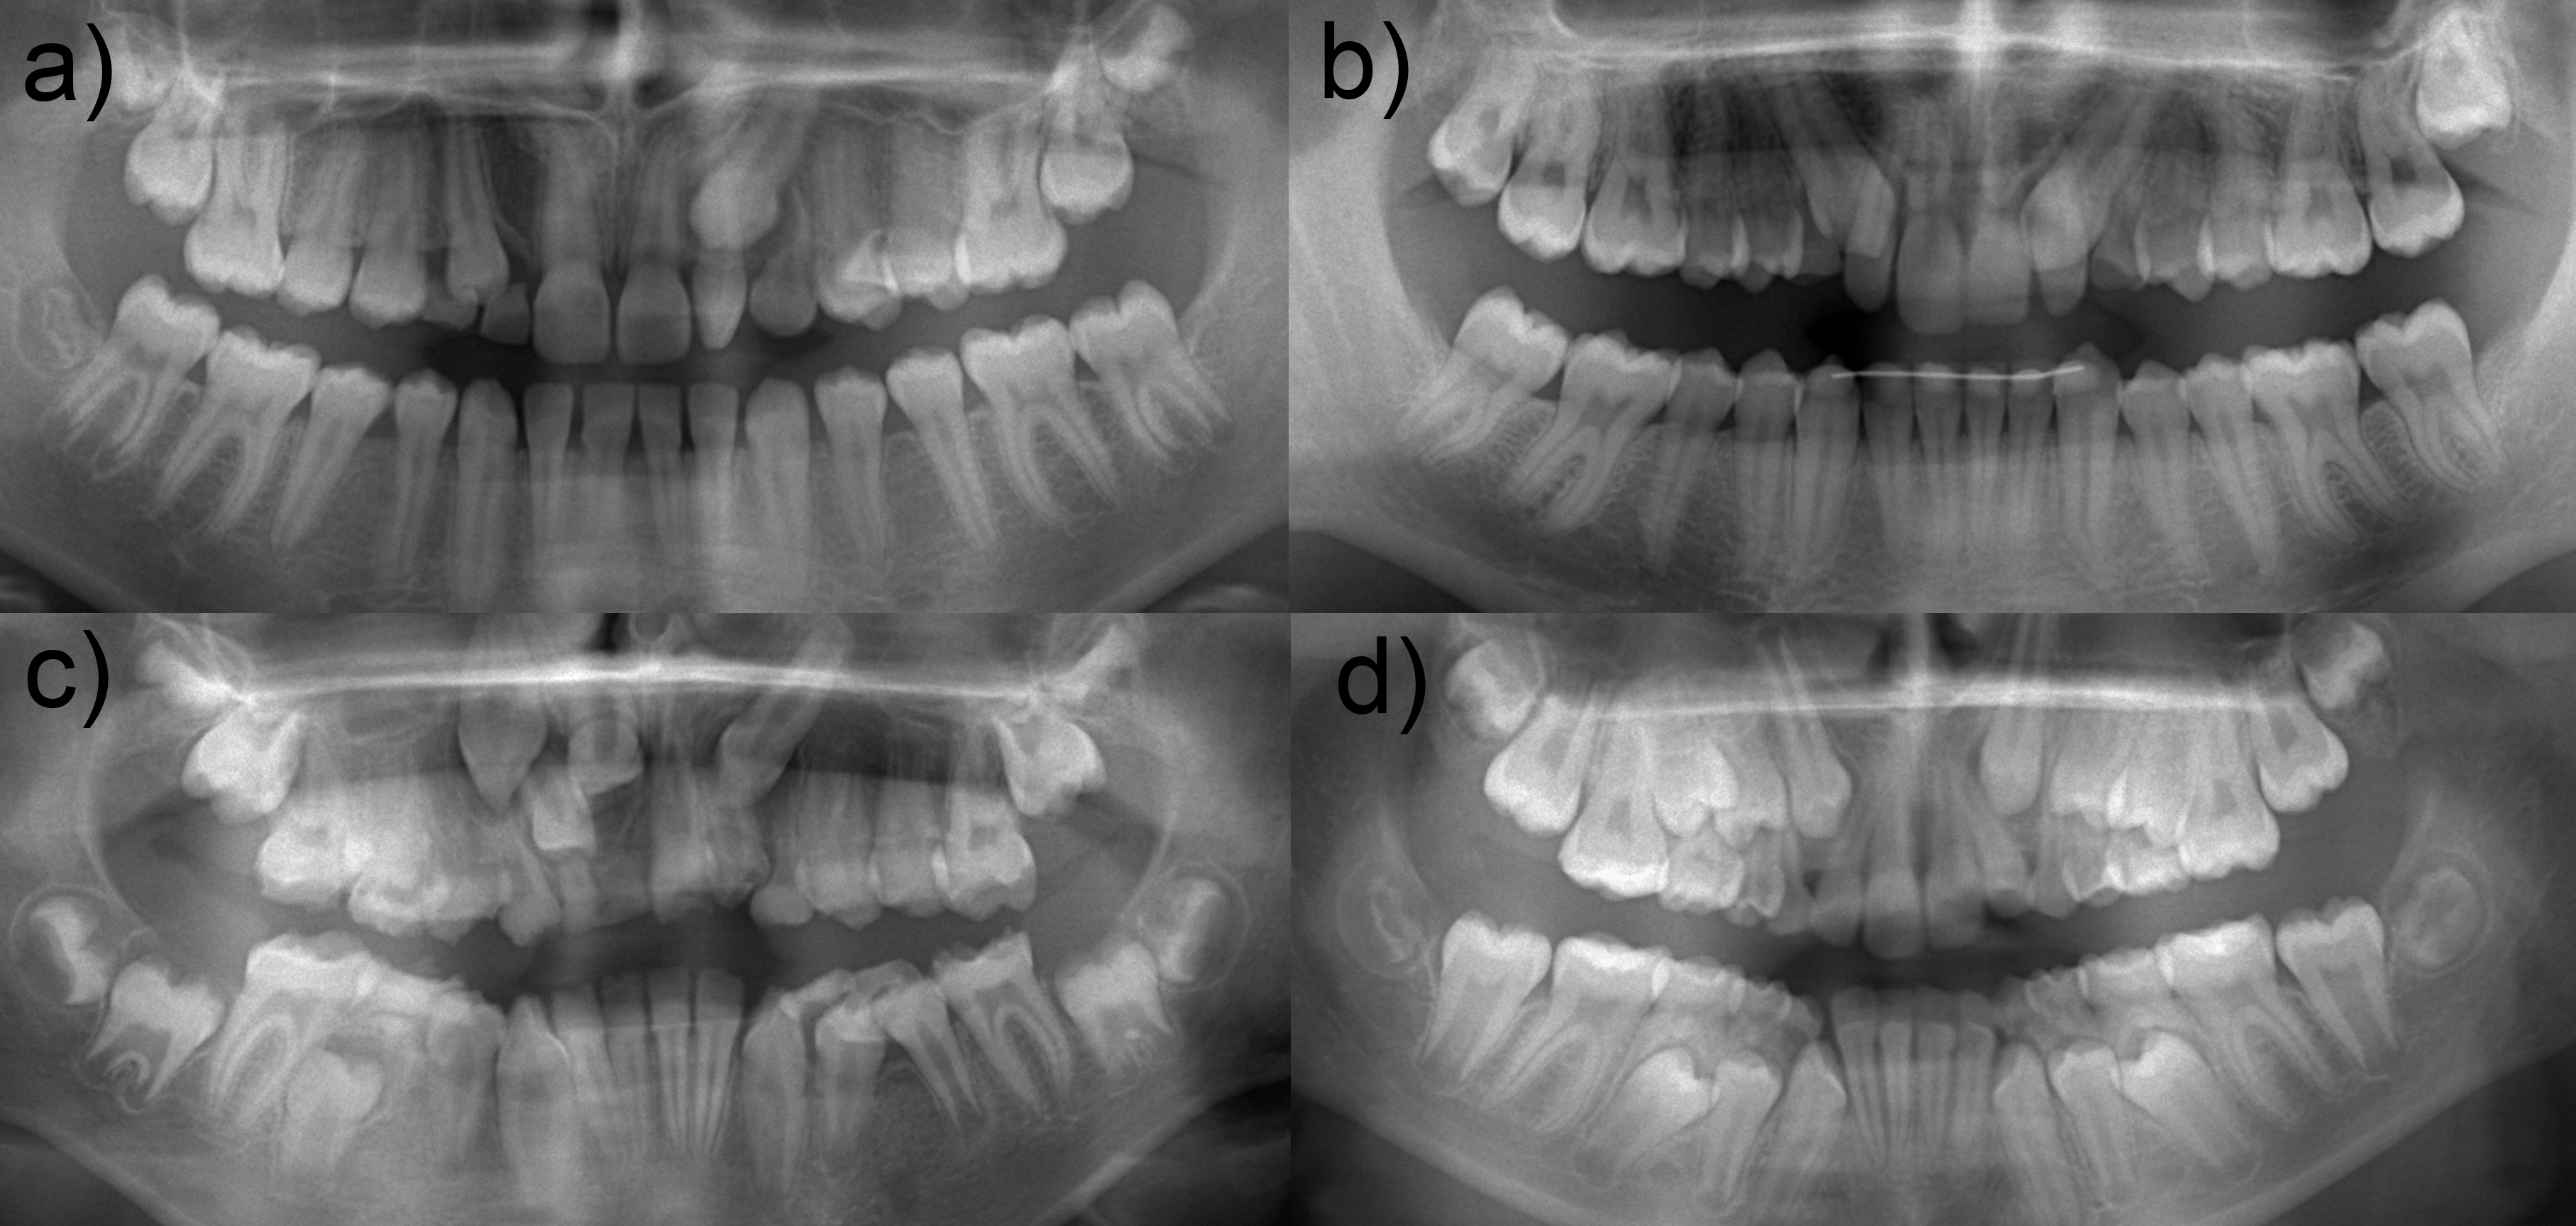
\includegraphics[width=0.95\columnwidth]{jaws.jpg}
\caption{Globally segmented jaws of test images a) 15, b) 17, c) 18, and d) 23.}
\label{jaws}
\end{figure}

The segmentation of the central teeth, however, presented some mistakes, as it was mentioned in subsection \ref{centralSegmentation}. Horizontally separating the upper and lower incisors was achieved in most of the occasions, but finding the actual central point of the jaw turned out to be quite difficult due to the variability in the vertical separation of the teeth. Since they are usually very close together (specially the ones of the lower jaw), segmenting them with adaptive thresholding not always yielded very good results. Figure \ref{jawSegmentation} already showed some examples of the optimal separation lines found by the algorithm, but Figure \ref{centralExamples} shows the final results of several of the test images. The algorithm found the center and segmented correctly the upper jaw of 68.75\% of the 16 test images, meanwhile the lower incisors were correctly segmented 87.5\% of the times, as can be seen in Table \ref{table1}, located in Appendix \ref{appendixA}.

\begin{figure}
\centering
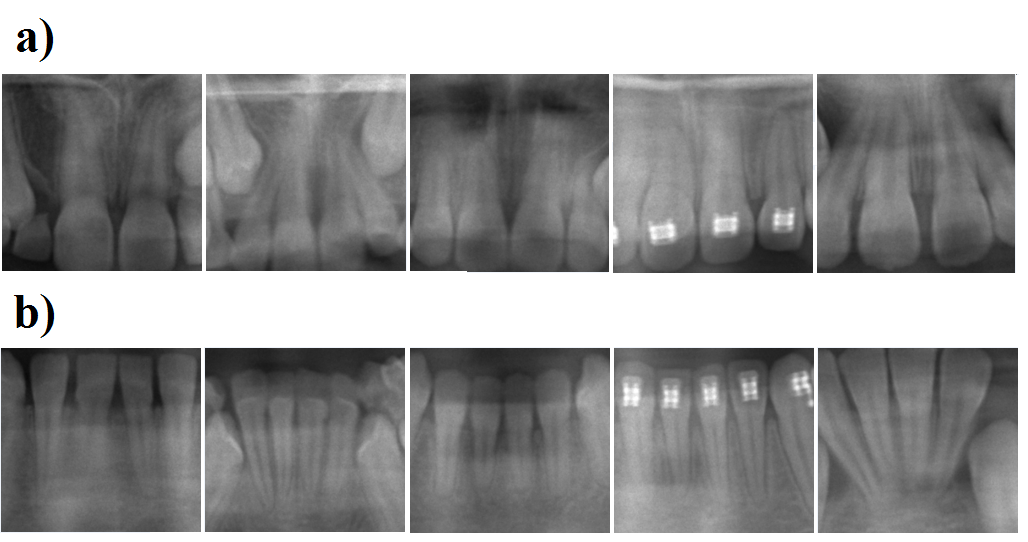
\includegraphics[width=0.95\columnwidth]{centralExamples.png}
\caption{Central segmentations by the method described in section \textsection\ref{centralTeeth} of a) the upper incisors and b) lower incisors of test images (from left to right) 15, 23, 24, 27, and 28.}
\label{centralExamples}
\end{figure}

After applying the ASM method, 62.5\% and 53.15\% of the upper and lower teeth, respectively, were approximately fitted (Table \ref{table2}, in Appendix \ref{appendixA}). However, if we are looking for a good, almost perfect match between the model shape and the actual tooth, the numbers decrease to 34.38\% for the upper incisors and 17.19\% for the lower incisors. Besides, it is important to take into account that some of the teeth were not segmented in the correct order. In certain occasions, during the fitting procedure, the model shape would migrate to another position and the segmented teeth were not exactly the incisors. In Figure \ref{finalSegmentation} that can be observed. This segmented teeth were the correct ones approximately 75\% of the times for the upper jaw and 50\% for the lower jaw. The difference is not surprising, considering that the lower incisors are much closer to each other and influence from the edges of neighboring teeth can make them migrate more easily. Taking into account this effect, we can roughly estimate that 25.79\% of the upper incisors would be almost perfectly fit, compared to 8.6\% of the lower ones.

\begin{figure}
\centering
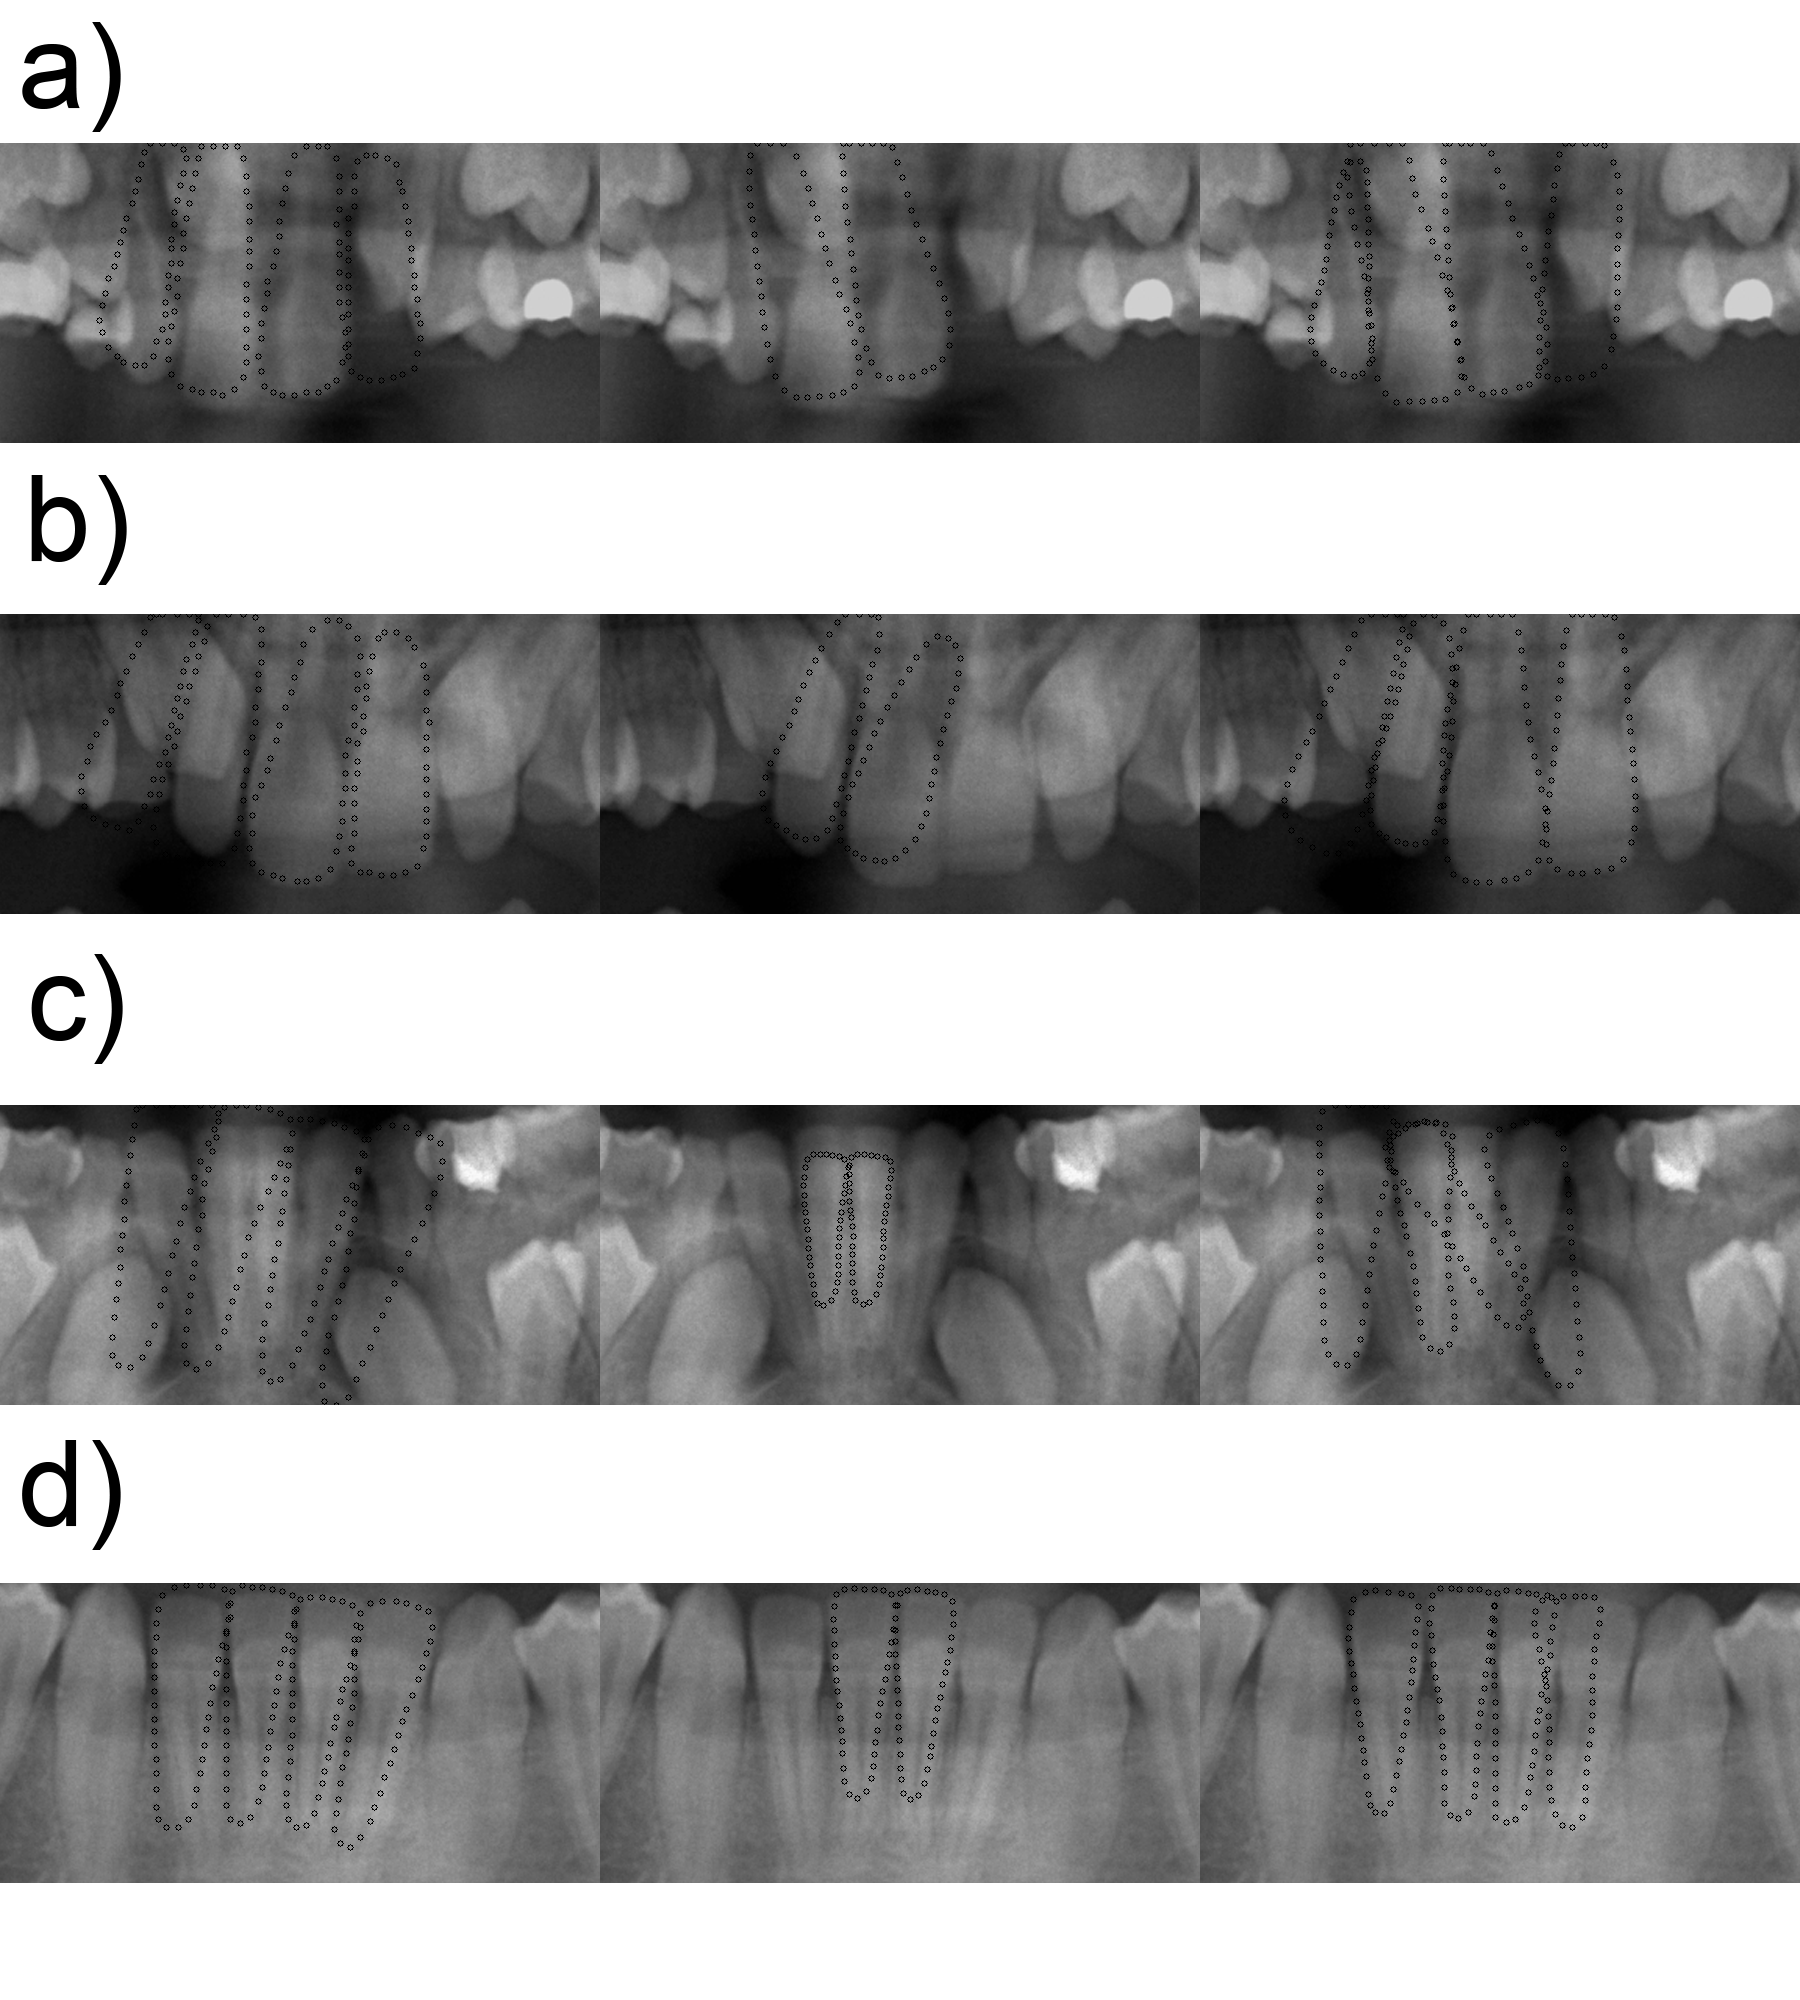
\includegraphics[width=0.95\columnwidth]{finalSegmentation.png}
\caption{Examples of different stages of the ASM algorithm for test images a) 16, b) 17, c) 26, and d) 30. From left to right: fitting of the the four teeth as a group, fitting of the two central incisors as a pair, and final result of the teeth being fitted individually. Notice the incorrect position of the model shape in b), the overlapping in the fittings in c), and how wrong intermediate steps can still lead to one or two correct segmentations. }
\label{finalSegmentation}
\end{figure}

Another reason for this effect could be a wrong segmentation of the central part of the jaw. It is interesting to compare the sources of errors. It was found that approximately 46.67\% of the mistakes (considering as a mistake a non-perfect segmentation or simply a failed one) in the upper jaw were most likely produced by the central segmentation procedure, compared to a 37.5\% for the lower teeth (Table \ref{table3}, in Appendix \ref{appendixA}). Accordingly, 53.33\% and 62.5\% of the times the error was probably produced by the ASM fitting. It is also interesting to note that it does not seem to be a strong relation between the sources of error of the lower and upper jaws of the same image, which could be due to the fact that the starting point of the ASM algorithm for the lower teeth takes feedback from the position of the upper ones. Also, most of the times that the fitting of all of the teeth fails, the source of error can be attributed to the central segmentation, which makes sense taking into account that the ASM needs a very precise starting point to be effective. It is to be noted that the sources of error cannot be always exactly determined, hence this information should be taken with caution.



\section{Conclusions and future work}\label{conclusions}

The algorithms proposed for incisor segmentations worked only on a limited number of test images. The jaw localization was proven to be effective, since it achieved a yield of 100\%. However, the implementation could be improved to take into account radiographs at different scales. Pyramidal representation is a widely used technique in image recognition that would easily solve this possible problem. 

Trying to segment the whole set of incisors presented several problems. Firstly, a binary image in which the teeth were represented by white pixels, meanwhile the background was kept black, was needed. This is a very difficult image to obtain, considering the great noise that is present in these kinds of radiographs. Many well-known techniques were applied in order to find a proper binary image in which the upper and lower teeth were segmented horizontally and laterally -- non-local means denoising, Canny edge detection, morphological dilation, iterative thresholding, and adaptive thresholding. Even so, the segmentation could not be properly made in many occasions. The main reason for this error is the necessity of obtaining an automated system to segment the incisors. If the images could be treated individually, one could find the perfect parameters for Canny edge detection or adaptive thresholding. However, since the algorithm should work for the highest number of radiographs possible, a trade-off needed to be found. A possible way of improving the performance of this algorithm would be allowing to rotate the image during the horizontal and vertical projections to achieve a better segmentation. Besides, different thresholding algorithms could be implemented.

The ASM used in this project also led to some wrong results, mainly from migration of the images due to the closeness of neighboring teeth. For example, the Mahanobis distance was found not to be useful in this case due to the fuzziness produced by other teeth and the wrong detection of edges in certain parts of the teeth. Again, these facts result from the optimization of trying to find the best preprocessing for all the images as a whole. In order to improve the segmentation and alleviate the effects of these sources of errors, extensive feedback was used during the procedure. Several teeth were fitted as a whole and their positions were used as inputs for the rest of the teeth. 

Many improvements could be made. With a larger database, it should be possible to improve the search of the center of the jaw using recognition of other teeth (e.g., the molars) as an input. Furthermore, after the first segmentation of the individual teeth, a smaller window could be constructed around a specific teeth and ASM could be applied again. In that manner, a more accurate fitting should be expected. The ASM could be modified to be more sophisticated. In order to prevent unwanted rotations of the model shape, constraints on the maximum rotation angle could be included. This constraint could be extracted from the Procrustes analysis of the set of landmarks provided, for example, taking the mean angle of the teeth. Another source of migration, specially of migration upwards (downwards), is a dragging of the image due to the influence of the many fuzzy edges found in the upper part (lower part). Adding weights that gave more importance to the parts of the teeth where true edges are usually found should make the stay in the correct position.


\newpage{}


\appendix

\section{Appendix: comparative tables}\label{appendixA}

\begin{table}[H]
\begin{center}
\begin{tabular}{|c| c| c |}
\hline
\textbf{Test image} & \textbf{Correct upper segmentation}  & \textbf{Correct lower segmentation}  \\ \hline
15 &  No, slightly lifted & Yes   \\
16 & Yes, but slightly off-center  & Yes \\ 
17 & No, right tooth cropped & Yes, but slightly off-center   \\ 
18 & Yes  & Yes, but off-center   \\  
19 & Yes & Yes   \\ 
20 & No, off-center, right tooth cropped & Yes, but slightly off-center   \\ 
21 & Yes & Yes   \\ 
22 & Yes, but right tooth slightly cropped & No   \\ 
23 & Yes & Yes   \\ 
24 & Yes & Yes   \\ 
25 & No, right tooth cropped & Yes   \\ 
26 & No, left tooth cropped & Yes, but off-center   \\ 
27 & Yes, but left tooth slightly cropped & Yes, but off-center   \\ 
28 & Yes & No   \\ 
29 & Yes, slightly off-center & Yes   \\ 
30 & Yes & Yes   \\ \hline 
Total & 68.75\% & 87.5\%  \\
\hline
\end{tabular}
\captionof{table}{Statistics of the performance of the central teeth segmentation algorithm. The row ``total'' reflects the percentage of correct segmentations.}\label{table1}
\end{center}
\end{table}

\begin{table}[H]
\begin{center}
\begin{tabular}{|c| cc c| cc c |}
\cline{2-7}
 \multicolumn{1}{c}{}&  \multicolumn{3}{|c|}{Upper teeth} & \multicolumn{3}{c|}{Lower Teeth} \\ \hline
\textbf{Image} & \textbf{Fitted}  & \textbf{Good match} & \textbf{Wrong teeth} & \textbf{Fitted}   & \textbf{Good match} & \textbf{Wrong teeth}  \\ \hline
15 &  3 & 3 & No & 2 & 0 & Yes  \\
16 & 4  & 1 & No & 0 & 0 &Yes \\ 
17 & 3 & 3 & Yes & 4 & 0 & Yes  \\ 
18 & 4  & 0 & No & 4 & 2 & No \\  
19 & 2 & 0 &  No  & 3 & 2 & No \\ 
20 & 3 &  2 & Yes & 2 & 2 & Yes  \\ 
21 & 3 & 0 & No & 0 & 0 & Yes  \\ 
22 & 1 & 1 & No & 0 & 0 & Yes  \\ 
23 & 0 & 0 & No  & 4 & 0 & No \\ 
24 & 3 & 1 & No  & 2 & 1 & No \\ 
25 & 0 & 0 & Yes  & 2 & 0 & Yes \\ 
26 & 2 & 1 & Yes & 1 & 1 & No  \\ 
27 & 3 & 2 & No  & 4 & 1 & No \\ 
28 & 4 & 4 & No & 0 & 0 & No  \\ 
29 & 2 & 0 & No  & 3 & 1 & Yes \\ 
30 & 3 & 3 & No & 3 & 1 & No  \\ \hline 
Total & 62.5\% & 32.81\% &  75\% & 53.13\% & 17.19\% &  50\% \\
\hline
\end{tabular}
\captionof{table}{Evaluation of the performance of the ASM algorithm. ``Fitted'' stands for number of fitted teeth and ``good match'' stands for an almost perfect match between model shape and teeth. ``Wrong teeth'' takes into account the times when the model shape was shifted and different teeth were segmented instead of the four incisors. The last row indicate the percentages of teeth fittings, almost perfect fittings and occasions where the segmented teeth were the correct ones.}\label{table2}
\end{center}
\end{table}

\begin{table}[H]
\begin{center}
\begin{tabular}{|c| c c| c c |}
\cline{2-5}
 \multicolumn{1}{c}{}&  \multicolumn{2}{|c|}{Upper teeth} & \multicolumn{2}{c|}{Lower Teeth} \\ \hline
\textbf{Test image} & \textbf{Mistakes}  & \textbf{Source of error} & \textbf{Mistakes}  & \textbf{Source of error}  \\ \hline
15 &  1 & Central segmentation & 4 & ASM  \\
16 &  3 & ASM & 4 & Central segmentation \\ 
17 & 4 & Central segmentation & 4 & Central segmentation  \\ 
18 & 4  & ASM & 2 & ASM \\  
19 & 4 & ASM  & 2 & ASM \\ 
20 & 4 & Central segmentation & 4 & Central segmentation  \\ 
21 & 4 & ASM & 4 & ASM  \\ 
22 & 1 & ASM & 4 & Central segmentation  \\ 
23 & 4 & Central segmentation  & 4 & ASM \\ 
24 & 3 & ASM  & 3 & ASM \\ 
25 & 4 & Central segmentation  & 4 & ASM \\ 
26 & 4 & Central segmentation & 3 & Central segmentation  \\ 
27 & 2 & ASM  & 3 & ASM \\ 
28 & 0 & -- & 4 & Central segmentation  \\ 
29 & 4 & Central segmentation  & 3 & ASM \\ 
30 & 1 & ASM & 3 & ASM  \\ \hline 
Central segmentation &  & 46.67\% & & 37.5\% \\ \hline
ASM & & 53.33\% & & 62.5\% \\
\hline
\end{tabular}
\captionof{table}{Estimation of the sources of error in the algorithm. ``Mistakes'' takes into account the amount of teeth that were wrongly segmented or that were segmented but in the wrong position (the model shape was shifted, see table \ref{table2}). The last two rows represent the percentage of times that each source of error was present. }\label{table3}
\end{center}
\end{table}

\section{Suplementary files}

This report should be accompanied by several folders and files. The function and behavior of each one of the Python files will be explained in Appendix \textsection\ref{python}. The folder called ``Report'' contains the Latex template of this file, together with the images and necessary files to generate the \textit{.pdf}. The folder ``\_Literature'' contains the bibliography used in this project. The folder called ``\_Data'' contains all the figures used in the folder ``Radiographs'' (train and test images) and the landmarks provided in ``Landmarks''. ``Segmentations'' is the final output of the algorithm, which has been moved to this location to make it easier to be found. The folder ``\_Data'' contains several images and subfolders, which are listed here:

\begin{itemize}

\item The 14 training images that were used are contained in the interior of this folder, with extension \textit{.tif}. This folder also contains three subfolders: ``extra'', ``PositiveJaws'' and ``NegativeJaws''.
\item ``PositiveJaws'' and ``NegativeJaws'' enclose the images used as positive and negative database, respectively, during the global segmentation of the jaw, as described in Section \textsection\ref{global}. The positive database is uniquely formed out of the manually cropped jaws of the 14 training images. The negative database, however, consists of several pictures of the non-jaw images.
\item The folder ``extra'' contains the 16 test images, with extension \textit{.tif}, and several subfolders. ``DenoisedFull'', ``DilationFull'' and ``EdgesFull'' contain the result of applying non-local means denoising, Canny edge detection and morphological dilation, respectively, used to find the appropiate parameters for this kind of images. 
\item The folder ``Cropped'' encloses the cropped version of the 16 test images, after applying the algorithm in Section \textsection\ref{global}, using the ``PositiveJaws'' and ``NegativeJaws'' databases. 
\item Within this folder, ``Preprocess'' contains the intermediate steps in the preprocessing of the image in order to find the best central segmentation of the teeth. This includes denoising, Canny edge detection, iterative thresholding, adaptive thresholding, and masking of the images to understand the output. The final results of the central segmentation, as described in Section \textsection\ref{centralTeeth} can be found in ``lowerTeeth'' and ``upperTeeth''. Both folders contain 4 images per test radiograph: the result of the lateral segmentation, the intermediate hypothesis in the incisor segmentation, the vertical separation of the teeth from this hypothesis image, and the final segmentation of the incisors.
\item Finally, the last two folders show the main results of the algorithm. ``incisorFitting'' contains all the fittings produced by the ASM approach described in Section \textsection\ref{ASM}, including the intermediate steps. The folder ``finalSegmentations'' contains binary images that represent the positions of the segmented incisors individually from the pictures of the cropped jaw. This is the folder where the final output of the algorithm is produced. This folder has also been copied with the name ``Segmentations'' in the folder ``\_Data''.
\end{itemize}

\section{Instructions to run the code}\label{python}

This project was developed using Python. The present section gives some instructions to compile all the program files in the corresponding order and understand their behavior. However, many comments can be found inside each one of the files, with the hope of providing some aclarations. Please, note that most of the code is not completely optimized. Many of the functions defined in some of the files can be also found in the rest. The reason for this is the fact that the codes were developed in parallel and many of the functions were re-used for several parts of the algorithm. This, of course, could have been avoided creating Python methods to call all the necessary functions. However, due to time issues, this could not be achieved. Also note that not all of the outputs produced are necessary for achieving the main function of the codes (segmenting the incisors), e.g., many images are shown in the screen but are not actually saved. The code is intended to be reviewed in every step, and for that reason extensive feedback is necessary. The files can be divided in three main parts: global segmentation of the jaw, segmentation of the incisors, and supplementary files. 

\subsection{Global segmentation}

The code dedicated to the segmentation of the incisors assumes that the images that are provided are already cropped and centered. Therefore, the file ``jaws.py'', which is in charge of finding and segmenting the jaw in a radiograph given an image file, should be run first. The main function of the code runs through the 16 files contained in the ``extra'' directory and applies the function ``findJaw'', which, as its name suggests, finds, segments and saves the cropped jaw image. This function, at the same time, makes use of many others,  which can also be found duplicated in the rest of the code. They are listed here:

\begin{itemize}
\item ``createX'' creates an array that contains all of the train images used for recognition.
\item ``pca'' performs a PCA of the train images and returns the eigenvectors, eigvenvalues and mean.
\item ``database'' resizes all of the positive and negative images to the same size and saves them in a ``rescaled'' directory.
\item ``project'' projects an image vector on the vectorial space spanned by the eigenvectors returned after  PCA and returns the coefficients.
\item ``reconstruct'' returns an image using the eigenvectors and the PCA coefficients obtained in ``project''.
\item ``normalize'' normalizes an image so that its maximum value is 255 and its minimum 0.
\item ``sliding\_window'' returns a window generator used for the recognition across the test image.
\end{itemize}

Finally, ``findJaw'' is the principal function of this file. The parameter ``show'' should be set True if the window search wants to be shown in screen. First, it loads the positive and negative databases, does PCA, and creates a sliding window. At each step of the search, it reconstructs the image using the positive and negative database and takes the Euclidean distance between the original image and the reconstructed one. The step size, as commented in Section \textsection\ref{global} is set to 8 pixels. A simple classifier  decides the class by selecting the reconstruction with the shorter distance to the original image. After the search, there are always several multidetections. The code tries to reduce the number of detections by exploring different algorithms, as explained in Section \textsection\ref{global}. The first two consist on clustering together the points that are below a certain threshold distance, following to different directions. The next one uses affinity propagation and then takes the median of all the clusters. Finally, the last part takes the median of all the originally detected windows, without applying any other algorithm, and saves the result. The intermediate steps are not useful for the final output, but are left in the code as illustration of the different possible approaches.

\subsection{Segmentation of the incisors}

If the code just described has been run, the cropped images should be found in the folder ``extra'', ready for the next part \footnote{Note that all of the inputs and outputs of every code file are already in the corresponding folders, so actually there is no need to run any part of the code}. The file ``mainMethod.py'' is in charge of the segmentation of all of the incisors, given the cropped jaw images in the folder ``extra''. 

\begin{enumerate}

\item First, it calculates the point where the upper teeth should be cropped in a window of a specified height and width. For that purpose, it uses the method ``segmentJaw''. This method has to functions, ``segmentLower'' and ``segmentUpper'', that segment separatedly the lower and upper incisors with the use of thresholding and intensity projections, as it was described in Section \textsection\ref{centralTeeth}.
\item Then, it fits the 4 teeth as a whole, in order to find the best general position, using the method ``fitAllCentralTeeth''. This method contains several functions:
\begin{itemize}
\item ``procrustesAnalysis'' and ``procrustes Rotation'' do a Procrustes analysis on the set of landmarks provided by centering, rescaling and aligning the rotation with respect to one of them, in order to be able to do a proper PCA.
\item ``normalize'' finds and return the normal vectors to the boundary in each one of the landmark points, used to find the maximum in the intensity profiles. This function takes into account the periodicity of the landmarks in each teeth and the fact that we are dealing with four different teeth.
\item ``getCentroid'' simply gets the central position of the set of 4 teeth.
\item ``findScalingRotation'' takes to images, X1 and X2, and tries to find the rotation, translation and scaling that best align both. One of the images would be the best fitting of the shape and the other one the suggested position of the landmarks, taking into account the maxima of intensity in the normal profiles.
\item ``getPCAcomponents'' is used to get the eigenvectors, eigenvalues and mean of a PCA using the landmarks of the 4 teeth as a whole of the 14 train images.
\item ``fitTeeth'' is the function called from ``mainMethod''. It takes the point where the image will be cropped with a certain height and width, the directory, a parameter ``wait'' that shows the fitting procedure step by step if set True, and ``lower'' that indicates if the fitting is made in the upper jaw, which could change the behavior slightly. This function loads all the landmarks, performs PCA, and calls the function ``activeShape'' with different scaling levels. After the fittings has been performed, it returns feedback of the center of each tooth, and the vector of fitted landmarks.
\item ``activeShape'' does the fitting of the shape. First, it takes the normal profile of each one of the landmarks and suggests a position depending on the intensity maxima of the edges. Then, it does a Procrustes analysis and a reconstruction with PCA of the ``most allowable'' shape that fits the model. Finally, it finds the best rotation, scaling and translation to fit the reconstructed landmarks with the suggested ones. If no convergence is found, the procedure is repeated.	
\end{itemize}
\item Next, using the feedback provided, it improves the position of the teeth and calculates the best fit. It performs a fit on the two central teeth and then on each tooth separately, using the methods ``fitCentralTeeth'' and ``fitOneTooth''. This two methods behave exactly the same as ``fitAllCentralTeeth'', but are optimized for 2 and 1 set of landmarks, respectively.
\item Finally, it segments the lower jaw, using feedback from the position of the upper incisors. This is done exactly the same as with the upper teeth.
\end{enumerate}

\subsection{Supplementary files}

The only two files that need to be run for to obtain the segmentations of the teeth are ``jaws.py'' and ``mainMethod.py'' (and if the jaws are already centered, only the latter). However, the following files might give some additional information:

\begin{itemize}
\item ``preprocessFull.py'' does a full preprocessing of any image in the specified directory. The preprocessing includes denoising, Canny edge detection and morphological dilation. This method can be used to quickly check the appropriate parameters for thresholding.
\item ``preprocess.py'' creates several files that contain comparisons between original, denoised, edge-detected, morphologically dilated, iteratively thresholded, adaptively thresholded, and masked images. This is useful to check the best parameters of thresholding to properly segment the central teeth.
\item ``fitAllCentralTeethMouse.py'' fits the four teeth as a whole taking as an input the center of the teeth selected with the mouse. This function can be used to improve the segmentation method easily and analyzing the importance of the starting point.
\item ``profiles.py'' saves in a directory plots of the profiles normal to the boundary of every landmark point. This file was used to check if the code was behaving correctly and the profiles were correct.
\end{itemize}

Finally, in the folder ``Junk code'' there are some additional files that contain pieces of code that were not finally used: ``molar.py'' and ``findIncisors.py''. These methods tried to find directly the position of the molar teeth and the incisors to get a good starting point for ASM using image recognition techniques. However, they were abandoned. The positive and negative databases necessary to run the files are not present.

\clearpage
\newpage

\begin{thebibliography}{11}
\bibitem{zhou}
Zhou, J., \& Abdel-Mottaleb, M. (2004, August). Automatic Human identification based on Dental X-ray images. In \textit{Defense and Security} (pp. 373-380). International Society for Optics and Photonics.
\bibitem{jain}
Jain, A. K., \& Chen, H. (2004). Matching of dental X-ray images for human identification. \textit{Pattern recognition, 37}(7), 1519-1532.
\bibitem{shah}
Shah, S., Abaza, A., Ross, A., \& Ammar, H. (2006, September). Automatic tooth segmentation using active contour without edges. In \textit{Biometric Consortium Conference, 2006 Biometrics Symposium: Special Session on Research at the} (pp. 1-6). IEEE.
\bibitem{sherif}
Al-sherif, N., Guo, G., \& Ammar, H. H. (2012, December). A New Approach to Teeth Segmentation. In \textit{Multimedia (ISM), 2012 IEEE International Symposium on} (pp. 145-148). IEEE.
\bibitem{nomir}
Nomir, O., \& Abdel-Mottaleb, M. (2005). A system for human identification from X-ray dental radiographs. \textit{Pattern Recognition, 38}(8), 1295-1305.
\bibitem{nonLocalMeans}
Buades, A., Coll, B., \& Morel, J. M. (2005, June). A non-local algorithm for image denoising. In \textit{Computer Vision and Pattern Recognition, 2005. CVPR 2005. IEEE Computer Society Conference on} (Vol. 2, pp. 60-65). IEEE.
\bibitem{openCV}
OpenCV library for python: http://opencv.org/
\bibitem{canny}
Canny, J. (1986). A computational approach to edge detection. \textit{Pattern Analysis and Machine Intelligence, IEEE Transactions on,} (6), 679-698.
\bibitem{adaptive}
Parker, J. R. (2010). \textit{Algorithms for image processing and computer vision.} John Wiley \& Sons.
\bibitem{ASM}
Cootes, T. F., Taylor, C. J., Cooper, D. H., \& Graham, J. (1995). Active shape models-their training and application. \textit{Computer vision and image understanding, 61}(1), 38-59.
\bibitem{ASM2}
Cootes, T., Baldock, E. R., \& Graham, J. (2000). An introduction to active shape models. \textit{Image Processing and Analysis,} 223-248.
\bibitem{mahalanobis}Mahalanobis, P. C. (1936). On the generalized distance in statistics. \textit{Proceedings of the National Institute of Sciences (Calcutta), 2,} 49-55.



\end{thebibliography}
\end{document}
